\renewcommand{\theequation}{\theenumi}
\begin{enumerate}[label=\arabic*.,ref=\thesubsection.\theenumi]
\numberwithin{equation}{enumi}
\item The general equation of circle, 
\begin{equation} \label{eq:circ}
x^2+y^2+2gx+2fy+c=0
\end{equation}
whose centre is $\myvec{-g\\-f}$
The vector form is, \\
$\vec{x}^T\myvec{1&0\\0&1}\vec{x}+\myvec{2g&2f}\vec{x}+c=0$


\item Point $\vec{A}$ = $\myvec{4\\1}$ lies on the circle. So, point $A$ satisfies the equation \ref{eq:circ} \\
$\vec{\myvec{4\\1}}^T\myvec{1&0\\0&1}\vec{\myvec{4\\1}}+\myvec{2g&2f}\vec{\myvec{4\\1}}+c=0$ \\
\begin{equation} \label{eq:circ_1}
8g+2f+c+17=0
\end{equation}

\item Point $\vec{B}$ = $\myvec{6\\5}$ lies on the circle. So, point $B$ satisfies the equation \ref{eq:circ} \\
$\vec{\myvec{6\\5}}^T\myvec{1&0\\0&1}\vec{\myvec{6\\5}}+\myvec{2g&2f}\vec{\myvec{6\\5}}+c=0$ \\
\begin{equation} \label{eq:circ_2}
12g+10f+c+61=0
\end{equation}

\item  Centre $\myvec{-g\\-f}$ lies on the line $\myvec{4&1}\vec{x}=16$ \\
$\myvec{4&1}\vec{\myvec{-g\\-f}}=16$ \\
\begin{equation} \label{eq:circ_3}
4g+f+16=0
\end{equation}

\item Solving equations \ref{eq:circ_1}, \ref{eq:circ_2} and \ref{eq:circ_3} \\
$$ g = -3, f = -4, c = 15$$
$\implies$ Equation of the circle is $x^2+y^2-6x-8y+15=0$ \\ 
The vector form is 
$$\vec{x}^T\myvec{1&0\\0&1}\vec{x}+\myvec{-6&-8}\vec{x}+15=0$$

\item The circle in Fig.\ref{fig:circ_1} is generated using the following python code 
\begin{lstlisting}
codes/circle/circle.py
\end{lstlisting}

\begin{figure}[!ht]
\centering
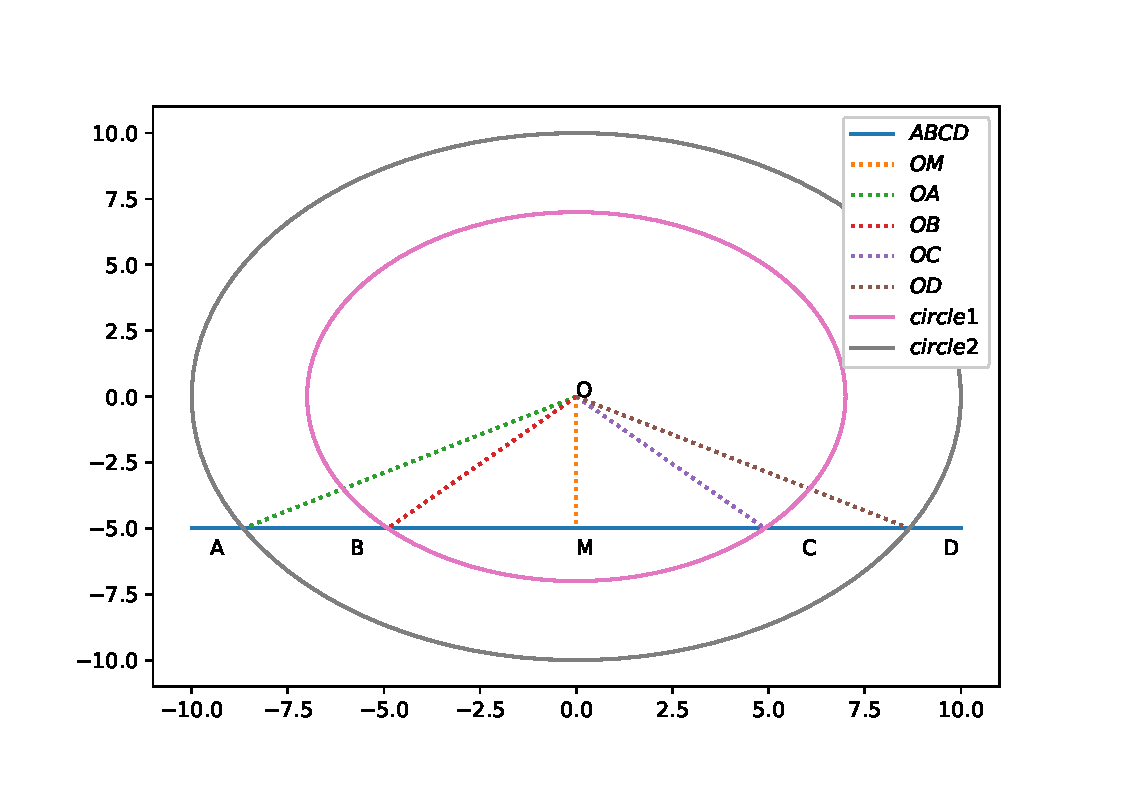
\includegraphics[width=\columnwidth]{./codes/circle/circle.eps}
\caption{Circle generated using python}
\label{fig:circ_1}
\end{figure}

\end{enumerate}